\documentclass{article}

% Language setting
% Replace `english' with e.g. `spanish' to change the document language
\usepackage[english]{babel}

% Set page size and margins
% Replace `letterpaper' with `a4paper' for UK/EU standard size
\usepackage[letterpaper,top=2cm,bottom=2cm,left=3cm,right=3cm,marginparwidth=1.75cm]{geometry}

% Useful packages
\usepackage{amsmath}
\usepackage{graphicx}
\usepackage[colorlinks=true, allcolors=blue]{hyperref}

\title{Exercise 1}
\author{Irma Hadzic 01428246}

\begin{document}
\maketitle
\begin{abstract}
    As a short summary, I chose to try to develop an model that can successfully clear one floor of the game Crypt of the Necrodancer. Crypt of the NecroDancer is a top down pixel rhythm game having a few inputs: up, down, left, right and consumables(bomb, item etc). It seemed simple enough to use for developing a reinforcement learning algorithm.
    \begin{figure}[h]
    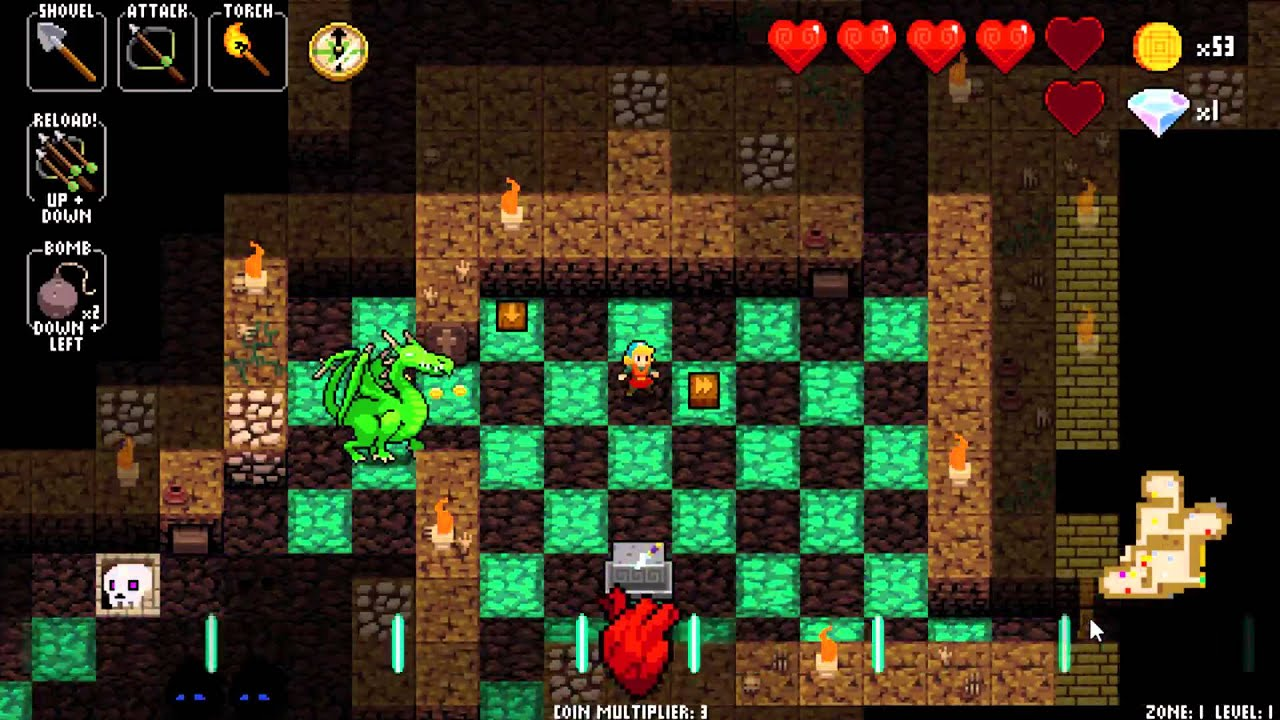
\includegraphics[width=8cm]{theCrypt.jpg}
    \centering
    \end{figure}
\end{abstract}

\section{References to at least two scientific papers that are related to your topic}
Here are the links to the related papers that I think will be really helpful in my project:
\begin{itemize}
    \item \href{https://paperswithcode.com/paper/playing-atari-with-deep-reinforcement}{Playing Atari with Deep Reinforcement Learning}
    \item \href{https://paperswithcode.com/paper/deep-reinforcement-learning-with-double-q}{Deep Reinforcement Learning with Double Q-learning}
    \item \href{https://bbukaty.github.io/CoNBot/report.pdf}{Crypt of the NecroDancer Bot}
    \item \href{https://informatika.stei.itb.ac.id/~rinaldi.munir/Citra/2019-2020/Makalah2019/13516002.pdf}{Feature Extraction From Crypt of the NecroDancer Interface
Using Hu Moments}
\end{itemize}

\section{A decision of a topic of your choice}
I chose the topic of Reinforcement Learning. As a complete beginner, it is really hard for me to understand how the theory can be put into practice. I see this project as an opportunity to answer this question in a way that is the most interesting to me: by playing games!
\section{A decision of which type of project you want to do}
I think my project will be in between "Bring your own data" and "Bring your own method". I think I need to implement a different model that would actually "learn" to play the game, and not just replicate human behavior. As I need a reward system, it can happen that a completely new dataset will be necessary to define what a reward is.
\section{A written summary that should contain:}
\subsection{Short description of your project idea}
 The project that I am mostly going to base my project on is \href{https://bbukaty.github.io/CoNBot/}{Crypt of the NecroDancer Bot} by Buck Bukaty and Amy Kanne. I want to develop a bot that can successfully clear the first floor of the crypt. The goal is not only kill all the monsters, but to also maximize the amount of gold collected. I am not sure if I am too ambitious for this project, so I will adapt after each step and set more realistic goals as I go.
\subsection{Description of the dataset you are about to collect}
As Buck and Amy describe it, I suppose my data is going to be "a dataset of recorded human gameplay" that consists "of screen captures of the game associated with the buttons that the human player was pressing"\cite{CotNDBot}. My goal is to exchange the human gameplay for a semi-automatic way to record machine gameplay, in order to train a model.
\subsection{A work-breakdown structure for the individual tasks}
First and foremost, I need to understand the code that is already provided on GitHub. The next matter of business is to be able to run the provided code on my PC. Next would be trying to implement some changes to the existing code for data recording, in order to introduce a suitable reward system. This reward system will then be used to try to change the model in such a way that it "learns" and not only replicates human behavior. As this is something I have never done before, I do not have a realistic timeframe in which all of these steps could be done.

\bibliographystyle{plain}
\bibliography{sample.bib}

\end{document}